\documentclass[11pt]{article}
\usepackage{amsmath, amssymb, amsthm}
\usepackage{geometry}
\usepackage{hyperref}
\usepackage{tikz}
\usetikzlibrary{arrows.meta, positioning}
\geometry{margin=1in}

\title{Notes 07 \\ Review of Statistics: \\ Multivariable Analysis}
\author{DATA 000: Advanced Computational Methods in Education and the Social Sciences}
\date{Alexander \\ Spring 2026}

\begin{document}

\maketitle

\tableofcontents

\section{Introduction}

\textbf{Multivariable analysis} refers to statistical models that use two or more independent variables (predictors) to explain or predict a single outcome (dependent variable)\ [1][2][3]. This is common in education and social sciences, where outcomes are influenced by multiple factors.

\section{Multivariable vs. Multivariate}

\begin{itemize}
    \item \textbf{Multivariable analysis:} One outcome, multiple predictors (e.g., multiple regression, multiple logistic regression).
    \item \textbf{Multivariate analysis:} Multiple outcomes, possibly multiple predictors (e.g., MANOVA, canonical correlation).
\end{itemize}

\section{Multiple Linear Regression}

\subsection{Model}

\[
Y = \beta_0 + \beta_1 X_1 + \beta_2 X_2 + \cdots + \beta_p X_p + \varepsilon
\]
\begin{itemize}
    \item $Y$: continuous outcome
    \item $X_1, X_2, \ldots, X_p$: predictors
    \item $\beta_0$: intercept
    \item $\beta_1, \ldots, \beta_p$: regression coefficients
    \item $\varepsilon$: error term
\end{itemize}

\subsection{Interpretation}

Each $\beta_j$ represents the expected change in $Y$ for a one-unit increase in $X_j$, holding all other predictors constant.

\subsection*{Visualization: Regression Plane (3D Example)}
\begin{center}
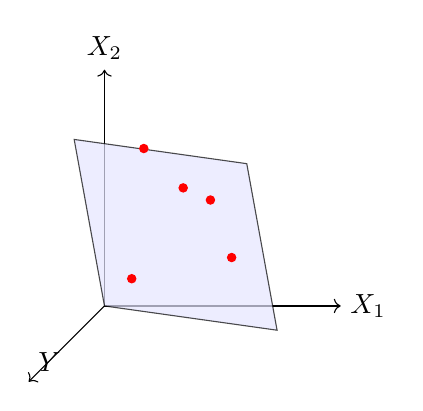
\begin{tikzpicture}[scale=1]
  % Axes
  \draw[->] (0,0,0) -- (3,0,0) node[right] {$X_1$};
  \draw[->] (0,0,0) -- (0,3,0) node[above] {$X_2$};
  \draw[->] (0,0,0) -- (0,0,2.5) node[above right] {$Y$};
  % Regression plane (approximate)
  \draw[fill=blue!10, opacity=0.7] (0,0,0) -- (2.5,0,0.8) -- (2.5,2.5,1.8) -- (0,2.5,1) -- cycle;
  % Example data points
  \foreach \x/\y/\z in {0.5/0.5/0.4, 2/1/1.0, 1.5/2/1.3, 2/2/1.7, 1/2.5/1.3} {
    \filldraw[red] (\x,\y,\z) circle (1.5pt);
  }
\end{tikzpicture}
\end{center}

\subsection{Example: Education (with Solution)}

\textbf{Scenario:} Predicting student GPA ($Y$) from hours studied per week ($X_1$) and number of absences ($X_2$):

\[
\text{Fitted model:} \quad \hat{Y} = 2.5 + 0.3 X_1 - 0.1 X_2
\]

\textbf{Interpretation:}
- Each additional hour studied increases GPA by 0.3, holding absences constant.
- Each additional absence decreases GPA by 0.1, holding study hours constant.
- A student who studies 10 hours/week and has 3 absences: $\hat{Y} = 2.5 + 0.3 \times 10 - 0.1 \times 3 = 2.5 + 3 - 0.3 = 5.2$ (if GPA scale allows).

\section{Multiple Logistic Regression}

\subsection{Model}

\[
\log\left(\frac{p}{1-p}\right) = \beta_0 + \beta_1 X_1 + \beta_2 X_2 + \cdots + \beta_p X_p
\]
\begin{itemize}
    \item $Y$: binary outcome (e.g., pass/fail)
    \item $p$: probability $Y=1$
    \item $X_1, X_2, \ldots, X_p$: predictors
\end{itemize}

\subsection{Interpretation}

Exponentiating a coefficient ($e^{\beta_j}$) gives the odds ratio for a one-unit increase in $X_j$, holding other variables constant.

\subsection*{Visualization: Logistic Surface (2 predictors)}
\begin{center}
\begin{tikzpicture}[scale=1]
  % Axes
  \draw[->] (0,0,0) -- (3,0,0) node[right] {$X_1$};
  \draw[->] (0,0,0) -- (0,3,0) node[above] {$X_2$};
  \draw[->] (0,0,0) -- (0,0,2.5) node[above right] {Probability};
  % Logistic surface (approximate curve)
  \draw[thick, blue] (0,0,0.1) -- (1,1,1.2) -- (2,2,2.1);
\end{tikzpicture}
\end{center}

\subsection{Example: Social Science (with Solution)}

\textbf{Scenario:} Predicting probability of voting ($Y=1$) from age ($X_1$) and education level ($X_2$):

\[
\log\left(\frac{p}{1-p}\right) = -2 + 0.05 X_1 + 0.3 X_2
\]

\textbf{Interpretation:}
- Each additional year of age increases odds of voting by $e^{0.05} \approx 1.05$.
- Each higher education level increases odds by $e^{0.3} \approx 1.35$.
- For a 40-year-old with education level 3:
\[
\text{Logit: } -2 + 0.05 \times 40 + 0.3 \times 3 = -2 + 2 + 0.9 = 0.9
\]
\[
\text{Odds: } e^{0.9} \approx 2.46 \implies p = \frac{2.46}{1+2.46} \approx 0.71
\]

\section{Model Diagnostics and Good Practices}

\subsection{Assumptions}

\begin{itemize}
    \item Linearity (for linear regression)
    \item Independence of errors
    \item No strong multicollinearity among predictors
    \item For logistic regression: linearity in the logit, no perfect separation
\end{itemize}

\subsection{Diagnostics}

\begin{itemize}
    \item \textbf{Residual plots:} Check for randomness (linear regression)
    \item \textbf{Variance Inflation Factor (VIF):} Assess multicollinearity
    \item \textbf{Hosmer-Lemeshow test:} Assess fit for logistic regression
    \item \textbf{$R^2$, Adjusted $R^2$}: Proportion of variance explained (linear regression)
    \item \textbf{AIC, BIC}: Model selection criteria
\end{itemize}

\section{Summary Table: Multivariable Models}

\begin{tabular}{|l|l|l|l|}
\hline
\textbf{Model} & \textbf{Outcome} & \textbf{Predictors} & \textbf{Interpretation} \\
\hline
Multiple Linear & Continuous & 2+ & Each $\beta_j$: change in $Y$ per unit $X_j$ \\
Multiple Logistic & Binary & 2+ & Each $e^{\beta_j}$: odds ratio for $X_j$ \\
\hline
\end{tabular}

\section{Further Notes}

\begin{itemize}
    \item Multivariable analysis is essential for controlling confounding and understanding complex relationships in observational data\ [1][2][3].
    \item Always check model assumptions and interpret results in the context of your research question.
    \item Software (R, Python, SPSS, Stata) is typically used for estimation.
\end{itemize}

\end{document}

